\documentclass[DIV=19,b5paper,twoside,12pt,spanish,russian,french,ngerman,latin,bahasai,english]{scrartcl}
\PassOptionsToPackage{english}{babel}
\PassOptionsToPackage{french}{babel}
\PassOptionsToPackage{ngerman}{babel}
\PassOptionsToPackage{latin}{babel}
\PassOptionsToPackage{bahasai}{babel}
\PassOptionsToPackage{russian}{babel}
\usepackage{hyperref}
\hypersetup{
pdftitle={Pentagame Regulae Rules Regeln Regles},
pdfsubject={Pentagame Rules in Many Languages},
pdfauthor={Jan Suchanek et al.},
pdfkeywords={Pentagame board game rules explained latin english german deutsch latine francais russian chinese spanish espaniol}
}
\usepackage{mathptmx}
\usepackage{babel}[ngerman,english,french,russian]
\usepackage[OT2,T1,T2A]{fontenc}
\usepackage[lutf8x,utf8]{luainputenc}
%\usepackage{ruhyphen}
\usepackage{setspace}
\usepackage{multicol}
\usepackage{titlesec}
\usepackage{microtype}
\usepackage{CJKutf8}
\usepackage{pgfpages,tikz,lipsum}
\usetikzlibrary{calc}
\usetikzlibrary{shapes.multipart}
\usetikzlibrary{arrows}
\usetikzlibrary{shapes.misc}
\usetikzlibrary{decorations.text}
\usetikzlibrary{automata, positioning}
\usetikzlibrary{hobby}
\usetikzlibrary{decorations.markings}
\usetikzlibrary{patterns}

%\usepackage{CJK}
\usepackage{tikz}
\raggedbottom
\raggedcolumns
\clubpenalty = 10000
\widowpenalty = 10000
\displaywidowpenalty = 10000

\newcommand{\noun}[1]{\textsc{#1}}




\makeatletter
\renewcommand\paragraph{%
\@startsection{paragraph}{4}%
{\z@}{1ex\@plus 1ex \@minus .2ex}%
{0.2ex \@plus .2ex}%
  {\sffamily\normalsize\bfseries}%
 }
 \makeatother


%%% Document specific commands

\newcommand{\myskip}{\smallskip}

\newcommand{\headline}{{\LARGE{}Pentagame}}
\newcommand{\tocent}{}
\newcommand{\translator}{}

\newcommand{\general}{}
\newcommand{\choosext}{}
\newcommand{\choosex}{}
\newcommand{\setupt}{}
\newcommand{\setup}{}
\newcommand{\objectivet}{}
\newcommand{\objective}{}
\newcommand{\rulest}{}
\newcommand{\rules}{}
\newcommand{\website}{\textsf{\textbf{pentagame.org}}}
\newcommand{\layout}{
\begin{centering}

{\sffamily\LARGE{\textbf\headline}}
\addcontentsline{toc}{section}{\tocent}

\end{centering}

\bigskip

\hrulefill


\begin{multicols}{2}

%\noindent\hrulefill
\general
\paragraph*{\choosext}
\choosex
\paragraph*{\setupt}
\setup
\paragraph*{\objectivet}
\objective


\medskip
\parbox{\columnwidth}{
\paragraph*{\rulest}
\rules
}

\end{multicols}}

\setlength{\parskip}{0ex}
\setlength{\parindent}{0cm}


\title{
\includegraphics[width=0.5\textwidth]{Pentagame_board_2018.png}\\
Penta$\cdot$game}
%\subtitle{by Jan Suchanek}
\author{ \href{mailto:jan@pentagame.org}{\makeatletter jan@pentagame.org\makeatother} }
\date{}

%% Actual Document. Calling the content first, then printing the same layout.

\begin{document}

\maketitle


 \begin{enumerate}
    \centering
        \item Every player has one piece on each corner
        \item Black blocks sit on central nodes
        \item Goal: Reach the coloured nodes opposite
        \item Everything goes, but no jumping allowed
        \item Replace blocks, swap with pieces
        \item Upon moving out, place a grey block
        \item Three pieces out wins
        \item Grey blocks are one time blocks
        \item No repetition (Ko)
    \end{enumerate}

%\tableofcontents

\newpage

\phantomsection
%\begin{multicols}{2}

\titlespacing*{\section}
{0pt}{1ex plus 1ex minus .2ex}{-2.3ex plus .2ex}
\newcommand{\skipper}{\medskip\hrulefill\section{}}

  
        \centering
        \includegraphics[width=0.5\textwidth]{Pentagame_board_2018.png}
        
        \vspace{6ex}
        
        {\sffamily\Large\textbf{PENTA$\cdot$GAME}}
        
        \bigskip

    \begin{enumerate}
    \centering
        \item Every player has one piece on each corner
        \item Black blocks sit on central nodes
        \item Goal: pieces want to reach the coloured nodes opposite
        \item Everything goes, but no jumping allowed
        \item Replace blocks, swap with pieces
        \item Upon moving out place a grey block
        \item Three pieces out wins
        \item Grey blocks are one time blocks
        \item No repetition (Ko)
    \end{enumerate}
    
\newpage



    \centering
    
    \skipper
    
    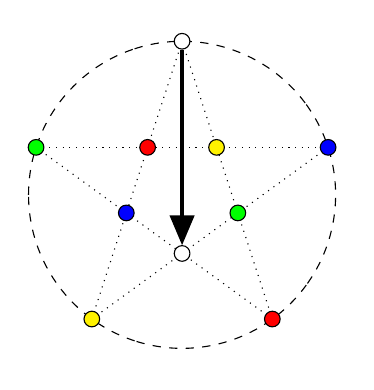
\begin{tikzpicture}[scale=0.65,state/.style={circle, draw, inner sep=2pt, opacity=1, fill=black, minimum size=0.2pt}]
    \tikzset{empty/.style={circle, draw, inner sep=2pt, opacity=0, fill=white, minimum size=0.2pt}}
    \tikzset{cross/.style={cross out, draw=black, minimum size=2*(#1-\pgflinewidth), inner sep=2pt, outer sep=2pt},
    %default radius will be 1pt. 
    cross/.default={1pt}}
    \scriptsize
    \begin{scope}[xscale=-1]
    \def \n {5} \def \radius {3cm} \def \raz {1.4cm}
    \foreach \s in {1,...,\n} { 
    \draw[dashed, >=latex] ({360/\n * (\s - 1)}:\radius)      arc ({360/\n * (\s - 1)}:{360/\n * (\s)}:\radius);   
    \draw[dotted, >=latex] ({360/\n * (\s - 2)+90}:\radius)      -- ({360/\n * (\s)+90}:\radius); 
    } 
    
    \node[state, fill=white] (1) at ({360/\n * (1 - 1)+90}:\radius) {};  
    \node[state, fill=white] (1a) at ({360/\n * (1 - 1)+90}:-\radius/2.618) {}; 
    
    \node[state, fill=blue] (2) at ({360/\n * (2 - 1)+90}:\radius){};   
    \node[state, fill=blue] (2a) at ({360/\n * (2 - 1)+90}:-\radius/2.618) {}; 
    
    \node[state, fill=red] (3) at ({360/\n * (3 - 1)+90}:\radius) {};  
    \node[state, fill=red] (3a) at ({360/\n * (3 - 1)+90}:-\radius/2.618) {}; 
    
    \node[state, fill=yellow] (4) at ({360/\n * (4 - 1)+90}:\radius) {}; 
    \node[state, fill=yellow] (4a) at ({360/\n * (4 - 1)+90}:-\radius/2.618) {}; 
    
    \node[state, fill=green] (5) at ({360/\n * (5 - 1)+90}:\radius) {};   
    \node[state, fill=green] (5a) at ({360/\n * (5 - 1)+90}:-\radius/2.618) {}; 
    
    
    \draw[>=triangle 45, line width=1.5pt, ->] (1) -- (1a);
    \end{scope}
    \end{tikzpicture}
    %\caption{Objective}
    
    You have five pieces.
    
    Bring them to the their \textbf{goals opposite their origins:}
    
    White to white, blue to blue etc.
    
    \textbf{Three out wins.}

% \begin{multicols}{2}
% \raggedcolumns



 
  
\skipper 

    \begin{tikzpicture}[scale=0.65,state/.style={circle, draw, inner sep=2pt, opacity=1, fill=black, minimum size=0.2pt}]
    \tikzset{empty/.style={circle, draw, inner sep=2pt, opacity=1, fill=white, minimum size=0.2pt}}
    \tikzset{cross/.style={cross out, draw=black, minimum size=2*(#1-\pgflinewidth), inner sep=2pt, outer sep=2pt},
    %default radius will be 1pt. 
    cross/.default={1pt}}
    \scriptsize
    \begin{scope}[xscale=-1]
    \def \n {5} \def \radius {3cm} \def \raz {1.4cm}
    \foreach \s in {1,...,\n} { 
    \draw[dashed, >=latex] ({360/\n * (\s - 1)}:\radius)      arc ({360/\n * (\s - 1)}:{360/\n * (\s)}:\radius);   
    \draw[dotted, >=latex] ({360/\n * (\s - 2)+90}:\radius)      -- ({360/\n * (\s)+90}:\radius); 
    } 
    %\draw[dashed] ({360/\n * (1 - 1)+95}:\radius)      arc ({360/\n * (1 - 1)+95}:{360/\n * (1)+85}:\radius)  node[midway, rotate=-18] {$\times$};
    \draw[>=triangle 45, line width=1.5pt, ->] ({360/\n * (1-1)+95}:\radius)  arc ({360/\n * (1-1)+95}:{360/\n * (2-1)+80}:\radius) node[midway,left]{};
    
    \draw[>=triangle 45, line width=1.5pt, ->] ({360/\n * (1-1)+95}:\radius)  arc ({360/\n * (1-1)+95}:{360/\n * (-1)+100}:\radius) node[midway,left]{};
    
    \draw[>=triangle 45, line width=1.5pt, shorten >=1.5ex, ->] (1) -- (4a);
    
    \draw[>=triangle 45, line width=1.5pt, shorten >=1.5ex, ->] (1) -- (3a);
    
    
    \node[state, fill=white] (1) at ({360/\n * (1 - 1)+90}:\radius) {};  
    \node[state, fill=white] (1a) at ({360/\n * (1 - 1)+90}:-\radius/2.618) {}; 
    
    \node[state, fill=blue] (2) at ({360/\n * (2 - 1)+90}:\radius){};   
    \node[state, fill=blue] (2a) at ({360/\n * (2 - 1)+90}:-\radius/2.618) {}; 
    
    \node[state, fill=red] (3) at ({360/\n * (3 - 1)+90}:\radius) {};  
    \node[state, fill=red] (3a) at ({360/\n * (3 - 1)+90}:-\radius/2.618) {}; 
    
    \node[state, fill=yellow] (4) at ({360/\n * (4 - 1)+90}:\radius) {}; 
    \node[state, fill=yellow] (4a) at ({360/\n * (4 - 1)+90}:-\radius/2.618) {}; 
    
    \node[state, fill=green] (5) at ({360/\n * (5 - 1)+90}:\radius) {};   
    \node[state, fill=green] (5a) at ({360/\n * (5 - 1)+90}:-\radius/2.618) {}; 
    
    \end{scope}
    \end{tikzpicture}
    %\caption{Simple move on ring}
    
    You can move \textbf{in any direction,} on the ring, on the star, clockwise, counter-clockwise, as you please.
    
   \skipper

  

    %%%% EXAMPLE MOVES
    \centering
    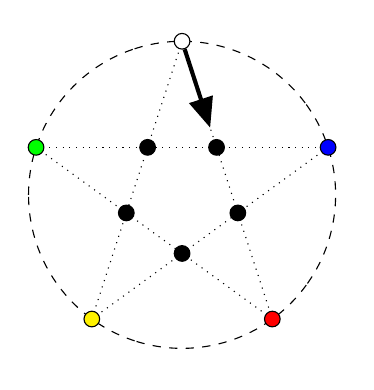
\begin{tikzpicture}[scale=0.65,state/.style={circle, draw, inner sep=2pt, opacity=1, fill=black, minimum size=0.2pt}]
    \tikzset{empty/.style={circle, draw, inner sep=2pt, opacity=0, fill=white, minimum size=0.2pt}}
    \tikzset{cross/.style={cross out, draw=black, minimum size=2*(#1-\pgflinewidth), inner sep=2pt, outer sep=2pt},
    %default radius will be 1pt. 
    cross/.default={1pt}}
    \scriptsize
    \begin{scope}[xscale=-1]
    \def \n {5} \def \radius {3cm} \def \raz {1.4cm}
    \foreach \s in {1,...,\n} { 
    \draw[dashed, >=latex] ({360/\n * (\s - 1)}:\radius)      arc ({360/\n * (\s - 1)}:{360/\n * (\s)}:\radius);   
    \draw[dotted, >=latex] ({360/\n * (\s - 2)+90}:\radius)      -- ({360/\n * (\s)+90}:\radius); 
    } 
    
    \node[state, fill=white] (1) at ({360/\n * (1 - 1)+90}:\radius) {};  
    \node[state, fill=black] (1a) at ({360/\n * (1 - 1)+90}:-\radius/2.618) {}; 
    
    \node[state, fill=blue] (2) at ({360/\n * (2 - 1)+90}:\radius){};   
    \node[state, fill=black] (2a) at ({360/\n * (2 - 1)+90}:-\radius/2.618) {}; 
    
    \node[state, fill=red] (3) at ({360/\n * (3 - 1)+90}:\radius) {};  
    \node[state, fill=black] (3a) at ({360/\n * (3 - 1)+90}:-\radius/2.618) {}; 
    
    \node[state, fill=yellow] (4) at ({360/\n * (4 - 1)+90}:\radius) {}; 
    \node[state, fill=black] (4a) at ({360/\n * (4 - 1)+90}:-\radius/2.618) {}; 
    
    \node[state, fill=green] (5) at ({360/\n * (5 - 1)+90}:\radius) {};   
    \node[state, fill=black] (5a) at ({360/\n * (5 - 1)+90}:-\radius/2.618) {}; 
    
    
    \draw[>=triangle 45, line width=1.5pt, shorten >=1.5ex, ->] (1) -- (4a);
    \end{scope}
    \end{tikzpicture}
    %\caption{Simple move}
    
    You can move \textbf{as far as you want.}
    
    But:\textbf{ you cannot jump!}
     

    
   
    \skipper
    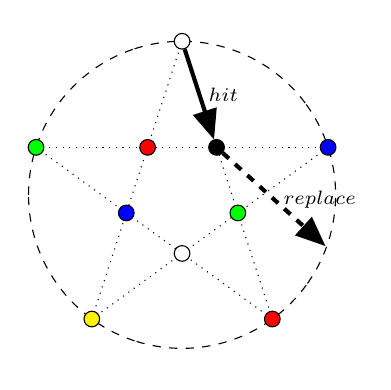
\begin{tikzpicture}[scale=0.65,state/.style={circle, draw, inner sep=2pt, opacity=1, fill=black, minimum size=0.2pt}]
    \tikzset{empty/.style={circle, draw, inner sep=2pt, opacity=1, fill=white, minimum size=0.2pt}}
    \tikzset{cross/.style={cross out, draw=black, minimum size=2*(#1-\pgflinewidth), inner sep=2pt, outer sep=2pt},
    %default radius will be 1pt. 
    cross/.default={1pt}}
    \scriptsize
    \begin{scope}[xscale=-1]
    \def \n {5} \def \radius {3cm} \def \raz {1.4cm}
    \foreach \s in {1,...,\n} { 
    \draw[dashed, >=latex] ({360/\n * (\s - 1)}:\radius)      arc ({360/\n * (\s - 1)}:{360/\n * (\s)}:\radius);   
    \draw[dotted, >=latex] ({360/\n * (\s - 2)+90}:\radius)      -- ({360/\n * (\s)+90}:\radius); 
    } 
    
    \node[state, fill=white] (1) at ({360/\n * (1 - 1)+90}:\radius) {};  
    \node[state, fill=white] (1a) at ({360/\n * (1 - 1)+90}:-\radius/2.618) {}; 
    
    \node[state, fill=blue] (2) at ({360/\n * (2 - 1)+90}:\radius){};   
    \node[state, fill=blue] (2a) at ({360/\n * (2 - 1)+90}:-\radius/2.618) {}; 
    
    \node[state, fill=red] (3) at ({360/\n * (3 - 1)+90}:\radius) {};  
    \node[state, fill=red] (3a) at ({360/\n * (3 - 1)+90}:-\radius/2.618) {}; 
    
    \node[state, fill=yellow] (4) at ({360/\n * (4 - 1)+90}:\radius) {}; 
    \node[state, fill=black] (4a) at ({360/\n * (4 - 1)+90}:-\radius/2.618) {}; 
    
    \node[state, fill=green] (5) at ({360/\n * (5 - 1)+90}:\radius) {};   
    \node[state, fill=green] (5a) at ({360/\n * (5 - 1)+90}:-\radius/2.618) {}; 
    
    
    \draw[>=triangle 45, line width=1.5pt, ->] (1) -- (4a) node[midway,right]{$hit$};
    
    \draw[dashed, >=triangle 45, line width=1.5pt, ->] (4a) -- (-2.8,-1) node[midway,right]{$replace$};
    
    \end{scope}
    \end{tikzpicture}
    %\caption{Replace a block}
    
    You can \textbf{hit a black block.} 
    
    You then \textbf{replace} it on another empty space.
    
    


  
    \skipper
    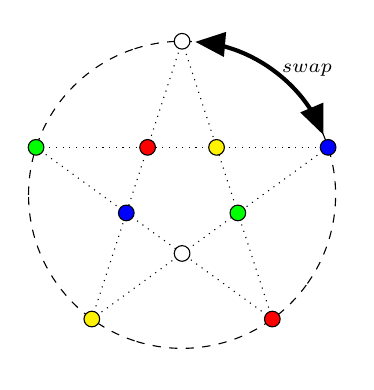
\begin{tikzpicture}[scale=0.65,state/.style={circle, draw, inner sep=2pt, opacity=1, fill=black, minimum size=0.2pt}]
    \tikzset{empty/.style={circle, draw, inner sep=2pt, opacity=1, fill=white, minimum size=0.2pt}}
    \tikzset{cross/.style={cross out, draw=black, minimum size=2*(#1-\pgflinewidth), inner sep=2pt, outer sep=2pt},
    %default radius will be 1pt. 
    cross/.default={1pt}}
    \scriptsize
    \begin{scope}[xscale=-1]
    \def \n {5} \def \radius {3cm} \def \raz {1.4cm}
    \foreach \s in {1,...,\n} { 
    \draw[dashed, >=latex] ({360/\n * (\s - 1)}:\radius)      arc ({360/\n * (\s - 1)}:{360/\n * (\s)}:\radius);   
    \draw[dotted, >=latex] ({360/\n * (\s - 2)+90}:\radius)      -- ({360/\n * (\s)+90}:\radius); 
    } 
    %\draw[dashed] ({360/\n * (1 - 1)+95}:\radius)      arc ({360/\n * (1 - 1)+95}:{360/\n * (1)+85}:\radius)  node[midway, rotate=-18] {$\times$};
    \draw[>=triangle 45, line width=1.5pt, <->] ({360/\n * (1-1)+95}:\radius)  arc ({360/\n * (1-1)+95}:{360/\n * (2-1)+85}:\radius) node[midway,right]{$swap$};
    
    %\draw[line width=1.5pt, -] ({360/\n * (1)+90}:\radius)      arc ({360/\n * (1)+90}:{360/\n * (2)+90}:\radius) node[midway,below]{};
    
    \node[state, fill=white] (1) at ({360/\n * (1 - 1)+90}:\radius) {};  
    \node[state, fill=white] (1a) at ({360/\n * (1 - 1)+90}:-\radius/2.618) {}; 
    
    \node[state, fill=blue] (2) at ({360/\n * (2 - 1)+90}:\radius){};   
    \node[state, fill=blue] (2a) at ({360/\n * (2 - 1)+90}:-\radius/2.618) {}; 
    
    \node[state, fill=red] (3) at ({360/\n * (3 - 1)+90}:\radius) {};  
    \node[state, fill=red] (3a) at ({360/\n * (3 - 1)+90}:-\radius/2.618) {}; 
    
    \node[state, fill=yellow] (4) at ({360/\n * (4 - 1)+90}:\radius) {}; 
    \node[state, fill=yellow] (4a) at ({360/\n * (4 - 1)+90}:-\radius/2.618) {}; 
    
    \node[state, fill=green] (5) at ({360/\n * (5 - 1)+90}:\radius) {};   
    \node[state, fill=green] (5a) at ({360/\n * (5 - 1)+90}:-\radius/2.618) {}; 
    
    \end{scope}
    \end{tikzpicture}
    %\caption{Swap two pieces}
    
    You can \textbf{swap} two neighbouring pieces \\ (at least one of which must be yours). 
    
    Of course the path must be free!
    
    
    
    

    %%%% TURN CORNERS
  
    \skipper
    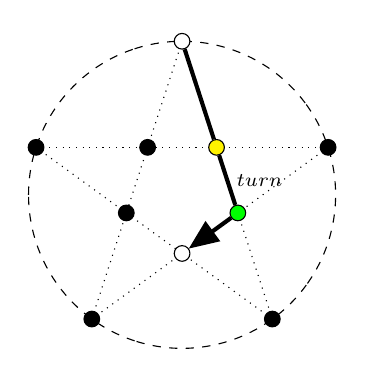
\begin{tikzpicture}[scale=0.65,state/.style={circle, draw, inner sep=2pt, opacity=1, fill=black, minimum size=0.2pt}]
    \tikzset{empty/.style={circle, draw, inner sep=2pt, opacity=1, fill=white, minimum size=0.2pt}}
    \tikzset{cross/.style={cross out, draw=black, minimum size=2*(#1-\pgflinewidth), inner sep=2pt, outer sep=2pt},
    %default radius will be 1pt. 
    cross/.default={1pt}}
    \scriptsize
    \begin{scope}[xscale=-1]
    \def \n {5} \def \radius {3cm} \def \raz {1.4cm}
    \foreach \s in {1,...,\n} { 
    \draw[dashed, >=latex] ({360/\n * (\s - 1)}:\radius)      arc ({360/\n * (\s - 1)}:{360/\n * (\s)}:\radius);   
    \draw[dotted, >=latex] ({360/\n * (\s - 2)+90}:\radius)      -- ({360/\n * (\s)+90}:\radius); 
    } 
    
    \node[state, fill=white] (1) at ({360/\n * (1 - 1)+90}:\radius) {};  
    \node[state, fill=white] (1a) at ({360/\n * (1 - 1)+90}:-\radius/2.618) {}; 
    
    \node[state, fill=black] (2) at ({360/\n * (2 - 1)+90}:\radius){};   
    \node[state, fill=black] (2a) at ({360/\n * (2 - 1)+90}:-\radius/2.618) {}; 
    
    \node[state, fill=black] (3) at ({360/\n * (3 - 1)+90}:\radius) {};  
    \node[state, fill=black] (3a) at ({360/\n * (3 - 1)+90}:-\radius/2.618) {}; 
    
    \node[state, fill=black] (4) at ({360/\n * (4 - 1)+90}:\radius) {}; 
    \node[state, fill=yellow] (4a) at ({360/\n * (4 - 1)+90}:-\radius/2.618) {}; 
    
    \node[state, fill=black] (5) at ({360/\n * (5 - 1)+90}:\radius) {};   
    \node[state, fill=green] (5a) at ({360/\n * (5 - 1)+90}:-\radius/2.618) {}; 
    
    
    \draw[>=triangle 45, line width=1.5pt, -] (1) -- (4a) node[midway,right]{};
    \draw[>=triangle 45, line width=1.5pt, -] (4a) -- (5a) node[midway,right]{$turn$};
    \draw[>=triangle 45, line width=1.5pt, ->] (5a) -- (1a) node[midway,left]{};
    
    \end{scope}
    \end{tikzpicture}
    \hspace{2ex}
    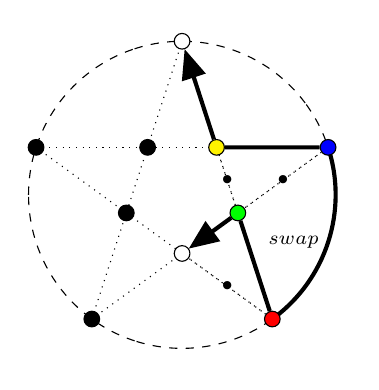
\begin{tikzpicture}[scale=0.65,state/.style={circle, draw, inner sep=2pt, opacity=1, fill=black, minimum size=0.2pt}]
    \tikzset{empty/.style={circle, draw, inner sep=2pt, opacity=1, fill=white, minimum size=0.2pt}}
    \tikzset{cross/.style={cross out, draw=black, minimum size=2*(#1-\pgflinewidth), inner sep=2pt, outer sep=2pt},
    %default radius will be 1pt. 
    cross/.default={1pt}}
    \scriptsize
    \begin{scope}[xscale=-1]
    \def \n {5} \def \radius {3cm} \def \raz {1.4cm}
    \foreach \s in {1,...,\n} { 
    \draw[dashed, >=latex] ({360/\n * (\s - 1)}:\radius)      arc ({360/\n * (\s - 1)}:{360/\n * (\s)}:\radius);   
    \draw[dotted, >=latex] ({360/\n * (\s - 2)+90}:\radius)      -- ({360/\n * (\s)+90}:\radius); 
    } 
    
    \draw[line width=1.5pt, -] ({360/\n * (1)+90}:\radius)      arc ({360/\n * (1)+90}:{360/\n * (2)+90}:\radius) node[midway,left]{$swap$};
    
    \node[state, fill=white] (1) at ({360/\n * (1 - 1)+90}:\radius) {};  
    \node[state, fill=white] (1a) at ({360/\n * (1 - 1)+90}:-\radius/2.618) {}; 
    
    \node[state, fill=blue] (2) at ({360/\n * (2 - 1)+90}:\radius){};   
    \node[state, fill=black] (2a) at ({360/\n * (2 - 1)+90}:-\radius/2.618) {}; 
    
    \node[state, fill=red] (3) at ({360/\n * (3 - 1)+90}:\radius) {};  
    \node[state, fill=black] (3a) at ({360/\n * (3 - 1)+90}:-\radius/2.618) {}; 
    
    \node[state, fill=black] (4) at ({360/\n * (4 - 1)+90}:\radius) {}; 
    \node[state, fill=yellow] (4a) at ({360/\n * (4 - 1)+90}:-\radius/2.618) {}; 
    
    \node[state, fill=black] (5) at ({360/\n * (5 - 1)+90}:\radius) {};   
    \node[state, fill=green] (5a) at ({360/\n * (5 - 1)+90}:-\radius/2.618) {}; 
    
    
    \draw[>=triangle 45, line width=1.5pt, <-] (1) -- (4a) node[midway,right]{};
    \draw[>=triangle 45, line width=1.5pt, -] (4a) -- (2) node[midway,left]{};
    \draw[>=triangle 45, line width=1.5pt, -] (3) -- (5a) node[midway,left]{};
    
    \draw[>=triangle 45, line width=1.5pt, ->] (5a) -- (1a) node[midway,left]{};
    
    \draw[dotted] (5a) --  (4a) node[midway, color=black] {$\bullet$};
    \draw[dotted] (2) --  (5a) node[midway, color=black] {$\bullet$};
    \draw[dotted] (3) --  (1a) node[midway, color=black] {$\bullet$};
    
    
    \end{scope}
    \end{tikzpicture}
    %\caption{Turn corners on free paths}
    
    \textbf{Turn} at free corners without stopping. 

    Paths can be long!
    
    \pagebreak
    

  
        \skipper
    %%%% EXAMPLE MOVES
    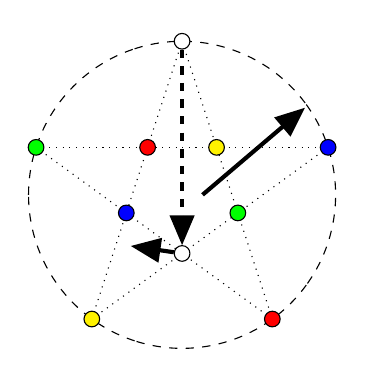
\begin{tikzpicture}[scale=0.65,state/.style={circle, draw, inner sep=2pt, opacity=1, fill=black, minimum size=0.2pt}]
    \tikzset{empty/.style={circle, draw, inner sep=2pt, opacity=0, fill=white, minimum size=0.2pt}}
    \tikzset{cross/.style={cross out, draw=black, minimum size=2*(#1-\pgflinewidth), inner sep=2pt, outer sep=2pt},
    %default radius will be 1pt. 
    cross/.default={1pt}}
    \scriptsize
    \begin{scope}[xscale=-1]
    \def \n {5} \def \radius {3cm} \def \raz {1.4cm}
    \foreach \s in {1,...,\n} { 
    \draw[dashed, >=latex] ({360/\n * (\s - 1)}:\radius)      arc ({360/\n * (\s - 1)}:{360/\n * (\s)}:\radius);   
    \draw[dotted, >=latex] ({360/\n * (\s - 2)+90}:\radius)      -- ({360/\n * (\s)+90}:\radius); 
    } 
    
    \node[state, fill=white] (1) at ({360/\n * (1 - 1)+90}:\radius) {};  
    \node[state, fill=white] (1a) at ({360/\n * (1 - 1)+90}:-\radius/2.618) {}; 
    
    \node[state, fill=blue] (2) at ({360/\n * (2 - 1)+90}:\radius){};   
    \node[state, fill=blue] (2a) at ({360/\n * (2 - 1)+90}:-\radius/2.618) {}; 
    
    \node[state, fill=red] (3) at ({360/\n * (3 - 1)+90}:\radius) {};  
    \node[state, fill=red] (3a) at ({360/\n * (3 - 1)+90}:-\radius/2.618) {}; 
    
    \node[state, fill=yellow] (4) at ({360/\n * (4 - 1)+90}:\radius) {}; 
    \node[state, fill=yellow] (4a) at ({360/\n * (4 - 1)+90}:-\radius/2.618) {}; 
    
    \node[state, fill=green] (5) at ({360/\n * (5 - 1)+90}:\radius) {};   
    \node[state, fill=green] (5a) at ({360/\n * (5 - 1)+90}:-\radius/2.618) {}; 
    
    
    \draw[dashed, >=triangle 45, line width=1.5pt, ->] (1) -- (1a);
    
    \draw[>=triangle 45, line width=1.5pt, ->] (1a) -- (1,-1);
    
    \draw[>=triangle 45, line width=1.5pt, ->] (-0.4,0) -- (-2.4,1.7);
    
    
    \end{scope}
    \end{tikzpicture}
    %\caption{Move out, set a new gray block}
    
    When you \textbf{reach a goal,} your piece moves \textbf{out. }
    
    For this you \textbf{place a grey block} anywhere.
    
    Grey blocks are \textbf{one-time blocks.}
    
    \skipper

\raggedright

\vspace{5ex}

Edge cases:

    \begin{enumerate}
        \item When moving to a corner with multiple pieces, swap with one of them.
        \item You can't try the same twice.
        \item When you get to set both a grey and a black block say `Abracadabra'.
        \item When you bring another player's piece to her goal she moves out once it's her turn.
        \item When you need more grey blocks than there are re-position one.
    \end{enumerate}

%\vfill

\skipper

\vspace{5ex}


You are welcome to visit \website ! 


%\end{multicols}

\clearpage

\selectlanguage{english}
\renewcommand{\headline}{Penta$\cdot$game - English}
\renewcommand{\tocent}{English}
\renewcommand{\translator}{Dr.~Robert Chapman}
\renewcommand{\general}{
A game that can be explained in a minute yet remains fascinating
for years.

 Two players play in just 20 minutes. Three or four players
may take up to 90. 

There are no dice involved. It is fine for all people from
age 5. A game by Jan \noun{Suchanek.}

In the box: 4$\times$5 coloured figures, 5 black and
5 gray blocks, the board.
}

\renewcommand{\choosext}{Choose your figures}
\renewcommand{\choosex}{
Every player has five figures. There is one team of figures per player in the box. 
%One team has silver hair, one team has black hair, one has golden hair and one is bald. 

%Players should play the team they look like. 

You have a blue, a red, a white, a green and a yellow figure. 

They start at the five corners of the board matching their colour.

They want to reach the big stops in the middle.
}
\renewcommand{\setupt}{Setup}
\renewcommand{\setup}{
Put your figures on the big corners at the ring matching their body colours: 
your white figure on the white corner at the ring, your blue figure on the blue corner at the ring, etc.

Put the black blocks on the five crossings in the middle of the board. 

Park the gray blocks in the middle for later. 
}

\renewcommand{\objectivet}{Objective}
\renewcommand{\objective}{
White figures want to go to the white crossing in the centre, blue
ones to the blue crossing, etc. The destination is always the big
coloured stop in the middle pentagon opposite the starting point.

Be the first to move \emph{three} pieces to their destinations to win.
}

\renewcommand{\rulest}{The Rules}
\renewcommand{\rules}{
Move any of your figures on the star or the ring in any direction as far as you please. 

You can turn at any free corner or crossing without stopping.

Never jump\textemdash neither over blocks, nor over any figures. 

\myskip

But you may move \emph{onto} a stop that is occupied:

\myskip

If you then beat a black block, place it on a free stop of your choice.

If you then move onto a stop with another figure, swap position with it.
 
\myskip

You may swap the positions of two of your own figures. 

If you move onto a stop with multiple figures, choose one to swap with.
 
\myskip 
 
Do not make the very same move twice in immediate succession.  

\myskip 

A figure that has reached its destination is removed. Put it into the centre of the board. Then take one of the gray blocks and put it on a free stop of your choice.

If you beat such a gray block, take it from the board again.

\myskip

Whoever moves \emph{three }of his figures out first wins.

\myskip

Excessive talking disqualifies.
}
\layout
\pagebreak

\selectlanguage{latin}
\renewcommand{\headline}{Penta$\cdot$ludus - Latine}
\renewcommand{\tocent}{Latine}
\renewcommand{\translator}{Dr.~J\"org Grimm / J.S.}
\renewcommand{\general}{ 

%\textbf{Descriptio }
Tabula pentagrammiforma, quattuor cohortes quinorum peditum coloratorum, quina impedimenta nigra et cana Pentaludum componunt. Fit Ioh.~\noun{Aridus.}

%\textbf{Cohortes }





}
\renewcommand{\choosext}{Cohortes}
\renewcommand{\choosex}{
Lusor quisque agit pedites quinos, quibus est eadem forma (aut stella aut luna \&c.), sed sunt diversi colores. 

Sic tua cohors peditem caeruleum, peditem rubrum  \&c. continet.

}

\renewcommand{\setupt}{Dispositio} 
\renewcommand{\setup}{ 
In quinque nodis positis in circulo, qui circumvenit pentagramma, ponite pedites eiusdem coloris: pedites albos in nodo albo, caeruleos
in nodo caeruleo \&c. 

Praeter illa decem loca quae nodos formant, existunt alter octoginta aedicula in viis, ubi pedites in ludo etiam possunt collocari. 

Sunt etiam impedimenta nigri et impedimenta cana. 

Impedimenta nigra ponite in nodis centri. In centro retinete impedimenta cana. 
}

\renewcommand{\objectivet}{Propositum} 
\renewcommand{\objective}{ 

Destinatio per unum quemque peditem, qui occupat nodum externi circuli, est nodus eiusdem coloris in interno pentagrammatis. 
Albo est eundum ad album, rubro ad rubrum \&c. 

Lusor victor qui primus duxit tres pedites ad nodum aequi coloris.

}

\renewcommand{\rulest}{Regulae } 
\renewcommand{\rules}{ 
Duc peditum tuorum unum in quamvis directionem sequens aut viam circuli aut vias stellae, quoad per regulas potes occupare aediculum. 

\myskip

In quodlibet aediculo libero, ubi  duae lineae conveniunt, tibi licet de via recta declinare sine retentione. 

\myskip

At numquam tibi licet transcendere nec impedimenta nec pedites alios.

\myskip

Potes vero ingredi in aediculum occupatum:

\myskip

Se ibi stat impedimentum nigrum, id pone in aediculo libero ad libitum. 

Se ibi iam stat pedes alius, pedites positiones suas mutare debent.

Se ibi sunt plures pedites (non potest fieri, nisi initio ludi), elige unum mutandum.

\myskip

Ita potes etiam mutare positiones duorum peditum tuorum.

\myskip

Bis eundem ne cana; eundem motum non licet iterum.

\myskip

Pedes progressus ad finem ludo abit. Pone eum in centrum.

Accipe per illo impedimentum canum et colloca in aediculo, quoad tibi paret. 

\myskip

Quando captas tale impedimentum canum, remove a tabula.

\myskip

Lusor  qui primus tres pedites ad finem duxit ludo victor.

\myskip

Gesta, non verba!
}
\layout
\pagebreak

\selectlanguage{ngerman}
\renewcommand{\headline}{Penta$\cdot$spiel - Deutsch}
\renewcommand{\tocent}{Deutsch}
\renewcommand{\translator}{J.S.}
\renewcommand{\general}{
Ein Spiel, das man in einer Minute begreift, das aber jahrelang fasziniert.

Zu zweit dauert die Partie nur 20 Minuten. Drei oder vier Spieler spielen 40-90 Minuten.

Es gibt keine Würfel. Geeignet für Spieler ab 5 Jahren. Ein Spiel von Jan  \noun{Suchanek.}

In der Schachtel: 4$\times$5 farbige Figuren, 5 schwarze und 5 graue Blöcke und das Spielbrett.
}

\renewcommand{\choosext}{Figuren}
\renewcommand{\choosex}{
Jeder Spieler führt eine Mannschaft von fünf Figuren.
%Da ist eine mit grauem, eine mit schwarzem, eine mit blondem und eine ohne Haar.

Jeder sucht sich eine Mann\-schaft aus.

In jeder solchen Mannschaft ist   eine blaue, eine rote, eine weiße, eine grüne und eine gelbe Figur.

Diese laufen alle von den fünf Ecken zu den fünf Kreuzungen.
}

\renewcommand{\setupt}{Aufbau}
\renewcommand{\setup}{
Stellt die Figuren geordnet nach Farben auf die fünf Ecken auf dem Kreis: die weißen auf das weiße Eckfeld, die blauen auf das blaue usw.

Je ein schwarzer Block kommt auf die Kreuzungen in der Mitte.

Die grauen Blöcke bleiben erst mal im Zentrum.
}

\renewcommand{\objectivet}{Ziel des Spiels}
\renewcommand{\objective}{
Weiße Figuren möchten zu der weißen Kreuzung, blaue zur blauen usw. 
Vom Rand her ist das Ziel immer die Kreuzung gleicher Farbe gegenüber.

Wer zuerst \emph{drei} seiner Figuren auf ihre jeweiligen Ziele zieht, gewinnt.
}

\renewcommand{\rulest}{Spielregeln}
\renewcommand{\rules}{
Ziehe eine deiner Figuren auf Stern oder Kreis in beliebiger Richtung so weit du kannst.

Du kannst dabei an jeder freien Kreuzung ohne anzuhalten abbiegen.

Du darfst ziehen, aber nicht springen! Weder über Blöcke noch über andere Figuren!

\myskip

Jedoch kannst du auf ein Feld ziehen das besetzt ist und schlagen:

\myskip

Schlägst du einen schwarzen Block, so setze ihn auf ein beliebiges freies Feld. 

Schlägst du eine andere Spielfigur, so tauschen deine und diese Figur ihre Positionen.

\myskip

Auf diese Weise kann man zwei seiner eigenen Figuren vertauschen.

Ziehst du auf ein Feld, auf dem noch mehrere Figuren stehen, musst du mit \emph{einer }von ihnen tauschen.
 
\myskip 
 
Man darf nicht denselben Zug zweimal machen. 

\myskip 

Hat eine Figur ihr Ziel erreicht, so zieht sie raus. Sie kommt ins Zentrum. Dafür darf man von dort einen grauen Block ins Brett auf ein freies Feld setzen.

Schlägt man so einen grauen Block, so kommt er wieder raus.


\myskip

Wer zuerst \emph{drei }seiner Figuren herauszieht, gewinnt. 

\myskip

Vorsagen ist verboten.
}

\layout
\pagebreak


%\selectlanguage{ngerman}
\renewcommand{\headline}{\section*{{\LARGE{}Penta$\cdot$spiel} - Vulgärdeutsch}}
\renewcommand{\general}{
N geiles Spiel, dasde inner Minute kapiern und jahrelang spieln kannst.

Zu zweit geht echt schnell, drei oder vier spieln länger.

Würfel gibts nich. Passt für alle ab 5. Von Jan.

In der Box sind 4 mal 5 Figuren, dann noch 5 schwarze und 5 graue Blöcke und das Brett.
}

\renewcommand{\choosex}{
\subsubsection*{Figuren}
Jeder hat ne Crew von fünf Figuren. Eine Crew hat graue Haare, eine hat schwarze usw., davon sucht sich jeder eine aus.

Dann hat jeder ne blaue, ne rote, ne weiße, ne grüne und ne gelbe Figur.

Alle laufen von den Ecken zu den bunten Kreuzungen.
}

\renewcommand{\setup}{
\subsubsection*{Aufbauen}
Stellt eure Leute je nach Farbe auf die fünf großen bunten Ecken am Rand: die weißen auf die weiße, die blauen auf die blaue usw.

Auf jede Kreuzung in der Mitte tustn schwarzen Block.

Die grauen Blöcke parkste erstmal im Zentrum.
}

\renewcommand{\objective}{
\subsubsection*{Worums geht}
Weiße wolln zur weißen Kreuzung, blaue zur blauen usw. Also das Ziel ist immer gegenüber. 

Wer das zuerst mit \emph{drei} Figuren hinkriegt, gewinnt.
}

\renewcommand{\rules}{
\subsection*{Spielregeln}
Du kannst laufen so weit und wolang du willst, bloß der Weg muss frei sein. 

Wenn frei ist kannste sogar abbiegen.

Aber überholen oder überspringen is nich!

\medskip

Schlagen kannste aber, und zwar so:

\medskip

N schwarzen Block kannste schlagen, dann tustn woanders hin.

Ne andere Spielfigur kannste auch schlagen, dann tauschste die zwei hin und her.

\medskip

So kannste auch zwei deiner eigenen Figuren swappen. 

Ziehste aufn Feld wo noch mehrere stehen, dann tauschte nur mit einer.

 
\medskip 
 
Genau dasselbe zweimal machen geht nich. 

\medskip 

Wennde ankommst, ziehste raus. Dafür kriechste n grauen Block, den kannste hintun wo du willst.

Schlägste so nen grauen Block so kommter wieder raus.


\medskip

Wer zuerst \emph{drei }rauszieht gewinnt. 

\medskip

Schnauze halten!
}

%\layout
%\pagebreak

\renewcommand{\headline}{Penta$\cdot$speel - Plattdüütsch}
\renewcommand{\tocent}{Plattdüütsch}
\renewcommand{\translator}{J.S.}
\renewcommand{\general}{
Kannst in een Minuut spitzkriegen liekers bleevt johrelang smakelk.

Twee Speler broken blots 20 Minuten. Dree or veer speeln 40-99 Minuten.

Wörpel gifft dat nich. Passlich för Speler af 5 Johren. En Speel vun Jan \noun{Suchanek}.

In de Lood: 4$\times$5 farvige Poppen, 5 swatte un 5 griese Blöck un de Speelbrett.
}

\renewcommand{\choosext}{Poppen}
\renewcommand{\choosex}{
Elk Speler föhrt en Koppel vun fief Poppen.

Jedereen söökt en so'n Koppel ut. 

In jede Koppel is 'ne blage, 'ne roote, 'ne witte, 'ne grööne un 'ne geele Popp. 

De trekken all vun de fief Ecken to de fief Krüüzen. 
}

\renewcommand{\setupt}{Opbuu}
\renewcommand{\setup}{

Stellt de Poppen no Forben ordnet op de fief Ecken op de Krink: de witten op de witte Eck, de blage op de blaage, usw. 

Op jedereen Krüüz kummt en swatte Block.

De griesen bleven iersmol in de Midd. 
}

\renewcommand{\objectivet}{Teel vun de Speel}
\renewcommand{\objective}{
Witte Poppen wulln to dat witte Krüüz, blaage to dat blaage, usw. 

Vun de Krink her is de Teel ümmer de Krüüz mit de sülve Farve op de günt siet. 

Welkeen toeerst \emph{dree} vun sünne Poppen op de rechte Teel trekkt, winnt.
}

\renewcommand{\rulest}{Regelwark}
\renewcommand{\rules}{
Treck een vun diene Puppen op de Stiern or de Krink as de möögst in elke Richt. 

An jedereen Krüüz kannst afbögen ahn stoppen. 

Du dörvst trekken, liekers nich jumpen! Kien över Blöck of över anner Poppen!

\myskip

Aver du kannst op een Feld trekken, dat besett is, un slaan:

\myskip

Slaagst du en swatten Block, sett eem up jichens en frieet Feld. 

Slaagst du en anner Popp, denn tuuschen de beeden Poppen de Steel.

\myskip

So kann man ook twee vun sünne egenen Poppen tuuschen.

Trekkst du op een Feld, op de noch veele Poppen stahn, muttst mit \emph{een }vun jüm tuuschen. 

\myskip 

Man dörv nich tweemol de sülven Treck maken. 

\myskip 

Kummt  en Popp to ehr Teel hen, trekkt se rut. Se kömmt in de Midd. Dorför kreegt man vun dor een griesen Block op en freet Feld to setten. 

Slaagt man so en griesen Block, kummt he wedder rut.

\myskip

Welkeen toeerst \emph{dree }vun sien Poppen uttrekkt, winnt. 

\myskip

Holl di stiev un sabbel keen dumm Tüüch!
}

\layout\
\pagebreak

\selectlanguage{french}
\renewcommand{\headline}{\section*{{\LARGE{}Penta$\cdot$jeux} - Fran\c{c}ais}}
\renewcommand{\tocent}{Fran\c{c}ais}
\renewcommand{\translator}{Armelle Journaix}
\renewcommand{\general}{ 
Un jeu de société qui s’explique en une minute mais reste fascinant pendant des années.

À deux, la partie dure environ 20 minutes. 
À trois ou quatre, la partie peut durer jusqu'à 90 minutes.

Aucun dé requis.
Âge : à partir de 5 ans. 
Par Jan \noun{Suchanek}.

Contenu de la boîte : 4 familles de 5 pions en couleurs, 5 pions noirs, 5 pions gris, un plateau.

}
\renewcommand{\choosext}{Choisissez vos pions}
\renewcommand{\choosex}{
Chaque joueur dispose de cinq pions.
Une famille est composée de cinq pions et il y en a cinq par joueur dans la boîte.

Il y a la famille aux cheveux argentés, la famille aux cheveux noirs, une famille aux cheveux dorés et une famille chauve.

Chaque équipe est composée de cinq pions : un bleu, un rouge, un blanc, un vert et un jaune.
}

\renewcommand{\setupt}{Installation}
\renewcommand{\setup}{ 
Disposez vos pions sur les cercles extérieurs correspondant aux couleurs des pions : votre pion blanc sur le cercle extérieur blanc, votre pion bleu sur le cercle extérieur bleu, etc.

Disposez les pions noirs sur les cercles intérieurs en couleurs.

Posez les pions gris au centre du plateau de jeu.
}

\renewcommand{\objectivet}{But du jeu}
\renewcommand{\objective}{
Les pions blancs doivent se rendre sur le cercle intérieur blanc, les pions bleus sur le cercle intérieur bleu, etc.

Le but est toujours le cercle intérieur coloré à l’opposé du cercle de départ.

Soyez le premier à déplacer trois de vos cinq pions sur leurs cercles intérieurs colorés respectifs pour gagner.
}

\renewcommand{\rulest}{Règles du jeu}
\renewcommand{\rules}{
Déplacez le pion de votre choix sur le plateau de jeu, où vous voulez et dans n'importe quelle direction.

Vous pouvez utiliser tous les chemins possibles.

Vous ne pouvez pas sauter les cercles occupés par des pions, quelle que soit leur couleur.

\medskip

Mais vous pouvez poser votre pion sur un cercle déjà occupé :

\medskip

Si vous posez votre pion sur un cercle occupé par un pion noir, prenez le pion noir et posez-le ensuite où vous voulez sur un cercle libre.

Si vous déplacez votre pion sur un cercle occupé par un autre pion, vous changez de place avec lui.

\medskip

Vous pouvez changer de place entre deux pions de votre famille.

Si vous déplacez votre pion sur une case occupée par plusieurs autres pions, choisissez-en un et changez de place avec lui.

\medskip

Vous ne pouvez pas effectuer le même déplacement deux fois de suite.

\medskip

Un pion qui atteint son but est retiré du jeu.

Ensuite, prenez l‘un des pions gris du centre du jeu et placez-le sur le cercle de votre choix.

Si votre pion se pose à la place d’un pion gris, le pion gris est retiré du jeu.

\medskip

Le premier joueur qui retire trois de ses pions du plateau gagne la partie.

\medskip

Parler excessivement vous disqualifie.
}
\layout
\pagebreak

\selectlanguage{russian}
\renewcommand{\headline}{\section*{{\LARGE{}Penta$\cdot$game} - Russian}}
\renewcommand{\tocent}{Русский}
\renewcommand{\translator}{alg}
\renewcommand{\general}{
Простая и интересная игра. Автор: Jan \noun{Suchanek}

Игра в среднем длится от 20 до 90 минут, в зависимости от количества игроков.

В коробке: 4$\times$5 разноцветных фигурок, 5 черных и
5 серых фигурок, игровое поле.
}

\renewcommand{\choosext}{Выбор фигурок}
\renewcommand{\choosex}{
Каждый игрок получает пять разноцветных фигурок одного типа.

Фигурки стартуют в вершинах пентаграммы.

Фигурки хотят достигнуть клетки в соответствующего цвета в середине поля.
}
\renewcommand{\setupt}{Подготовка}
\renewcommand{\setup}{

Расставьте фигурки в вершинах пентаграммы в соответствии с их цветом.

Расставьте черные фигурки на цветные клетки на пересечениях линий.

Поставьте серые фигурки в середину поля \textemdash  они понадобятся позже.

}

\renewcommand{\objectivet}{Цель}
\renewcommand{\objective}{
Выигрывает первый, кто переместит три фигурки в соответствующие их цвету клетки на пересечениях линий пентаграммы.
}

\renewcommand{\rulest}{Правила}
\renewcommand{\rules}{
В свой ход можно переместить любую свою фигурку на любое расстояние вдоль линий пентаграммы или кольца.

На развилках можно поворачивать без остановки.

Нельзя перепрыгивать через другие фигурки.

\medskip

Если остановиться \emph{на} занятой клетке:

\medskip

Если в клетке черная фигурка \textemdash переместите ее в любую свободную клетку.

Если в клетке фигурка, принадлежащая игроку \textemdash\ поставьте ее в клетку, в которой начинался ход.
 
\medskip

Если остановиться на клетке с несколькими фигурками \textemdash заместите одну из них.
 
\medskip 
 
Нельзя повторять один и тот же ход дважды.

\medskip 

Фигурка, достигнув назначенной клетки, удаляется с поля.
Игрок, которому принадлежит фигурка, взамен получает серую фигурку, которую можно поставить на любую свободную клетку.

При замещении, серая фигурка удаляется с поля.

\medskip

Во время игры нельзя болтать не по делу.
}

\layout
\pagebreak


\renewcommand{\headline}{Penta$\cdot$juego - Español}	
\renewcommand{\tocent}{Español}	
\renewcommand{\translator}{Juan José Bravo}	
\renewcommand{\general}{	
Un juego que se explica en un minuto pero que sigue fascinándote durante años.	
	
	
Una partida entre dos jugadores puede llevarte 20 minutos. Tres o cuatro jugadores pueden emplear hasta los 90 minutos.	
	
	
Requisitos: Se juega sin dados. A partir de cinco años.	
Realizado por  Jan \noun{Suchanek.}	
	
Contenido de la caja: 4 grupos de cinco peones de colores, 5 negros, 5 grises y un tablero.	
	
}		
	
\renewcommand{\choosext}{Elije tus peones}	
\renewcommand{\choosex}{	
Cada jugador dispone de cinco peones. Un equipo esta compuesta por cinco peones y hay cinco  por jugador en la caja. 	
%Hay un equipo con el  pelo plateado,un con pelo negro, otro rubio y otr sin pelo.	
	
%Los jugadores deben llevar el equipo que mas se les parezca. 	
	
Cada equipo esta compuesto por cinco peones; un peón azul, uno rojo, uno blanco, uno verde  y uno amarillo.	
	
Disponed vuestros peones en los círculos exteriores de los colores correspondientes:
Ellos tendrán que llegar a la meta situada en el medio del tablero. 	
}	

\renewcommand{\setupt}{Instalación}	
\renewcommand{\setup}{	
Disponed vuestros peones sobre los círculos exteriores en sus colores correspondientes: 
el peón blanco en el circulo exterior blanco, el azul en circulo exterior azul, etc.	
	
Dispón los peones negros en los cinco círculos interiores, en el medio del tablero.
Coloca los peones grises en el centro del tablero.	
}	
	
\renewcommand{\objectivet}{Objetivo}	
\renewcommand{\objective}{	
Los peones blancos deben alcanzar los círculos interiores blancos, los peones azules los círculos interiores azules, etc.	
El destino es siempre el gran circulo central de color en el medio del pentagama opuesto al punto de partida.	
	
	
Se el primero en colocar tres de tus cinco peones en los círculos de colores correspondientes para ganar.
}	
	
\renewcommand{\rulest}{Reglas del juego}	
\renewcommand{\rules}{	
Mueve el peón de tu elección sobre el tablero de juego, donde que quieras, sin importar la dirección, tan lejos como quieras.	
	
Tu puedes utilizar todos los caminos posibles.	
	
No podrás saltar sobre círculos ocupados.	
	
\myskip	
	
Pero podrás colocarte en un circulo  ocupado:	
	
\myskip	
	
Si caes en   un circulo ocupado por un peón negro, tomas este  y lo colocas en cualquier circulo libre, de tu elección.	
	
Si caes en un circulo ocupado por otro peón, cambias tu lugar anterior por el.	
	
\myskip	
	
Tu puedes cambiar  de posición entre dos peones de tu equipo. 	
	
Si caes en una casilla ocupada por varios peones, puedes elegir uno de ellos y cambiar de lugar con el.	
	
\myskip 	
	
No puedes hacer el mismo movimiento dos veces seguidas.	
	
\myskip 	
	
Cuando un peón llega a  la meta, es retirado del juego, se le coloca en el centro del tablero y se toma un peón gris que podrás colocar en cualquier circulo libre de tu elección.
	
Si caes en un lugar ocupado por un peón gris, este peón gris  sera retirado del juego.	
	
\myskip	
	
El primer jugador que consiga retirar tres peones ganará la partida.	
	
\myskip	
	
Hablar demasiado descalifica.

}


\layout
\pagebreak

\renewcommand{\headline}{Penta$\cdot$permeinan - Bahasa Indonesia}
\renewcommand{\tocent}{Bahasa Indonesia}
\renewcommand{\translator}{Iqbal Akbar, Sabrina Budiono}
\renewcommand{\general}{
Sebuah permainan yang dapat dijelaskan dalam satu menit tetapi tetap menarik selama bertahun-tahun. 

Dua pemain dapat bermain hanya dalam waktu 20 menit. Tiga atau empat pemain mungkin membutuhkan waktu hingga 90 menit.  

Permainan ini tidak membutuhkan dadu dan dapat dimainkan oleh semua orang mulai dari usia 5 tahun. Sebuah permainan oleh Jan \noun{Suchanek.}

Di dalam kotak: 4$\times$5 bidak berwarna, 5 kotak hitam dan
5 kotak abu-abu, papan permainan.
}

\renewcommand{\choosext}{Pilih Bidak Anda}
\renewcommand{\choosex}{
Setiap pemain memiliki 5 bidak. Di dalam kotak terdapat satu tim bidak untuk setiap pemain. 
%Satu tim memiliki bidak dengan rambut perak, satu dengan rambut hitam, satu dengan rambut emas, dan lainnya botak.

%Para pemain harus bermain tim yang mirip dengan mereka.

Anda memiliki bidak berwarna biru, merah, putih, hijau, dan kuning.

Para pemain memulai dari kelima sudut di papan permainan sesuai dengan warnanya.

Mereka harus mencapai tempat permberhentian di tengah papan permainan, dimana mereka keluar.
}

\renewcommand{\setupt}{Tata Permainan}
\renewcommand{\setup}{
Taruh bidak anda di sudut besar di sisi luar lingkaran, sesuai dengan warna bidak: bidak putih anda di sudut putih, bidak biru anda
di sudut biru, dan seterusnya.

Taruh blok hitam di lima persimpangan di tengah papan permainan.

Taruh blok abu-abu di tengah untuk tahap selanjutnya. 
}

\renewcommand{\objectivet}{Objektif}
\renewcommand{\objective}{
Bidak putih harus dimainkan menuju persimpangan berwarna putih di tengah, bidak
biru menuju persimpangan berwarna biru dan seterusnya. Tujuan akhirnya selalu
titik akhir di tengah, berlawanan dengan titik awal. 

Pemain pertama yang berhasil memindahkan \emph{three} bidak ke tujuan akhir adalah
pemenangnya.
}

\renewcommand{\rulest}{Peraturan}
\renewcommand{\rules}{
Pindahkan bidak anda ke bintang atau lingkaran ke berbagai arah dan jarak yang diinginkan. 

Anda bisa berbelok di sudut bebas atau persimpangan tanpa harus berhenti.

Jangan pernah lompat\textemdash melewati block ataupun bidak. 

\myskip

Tetapi anda diperkenankan berhenti \emph{di sana} jika tempat itu sudah terisi:

\myskip

Jika anda mengalahkan blok hitam, tempatkan blok tersebut ke tempat bebas sesuai pilihan anda.

Jika anda bergerak ke tempat yang terisi bidak lain, anda dapat bertukar posisi dengan bidak itu. 
 
\myskip

Anda diperkenankan menukar posisi dua bidak anda.  

Jika anda bergerak ke tempat dengan bidak lebih dari 1, pilih satu untuk ditukar. 
 
\myskip 
 
Jangan membuat gerakan yang sama dua kali setelah pergantian dadakan.   

\myskip 

Sebuah bidak yang mencapai titik akhir dipindahkan dan ditaruh di tengah papan permainan. Kemudian ambil satu blok abu-abu dan taruh di tempat bebas pilihan anda. 

Jika anda mengalahkan blok abu-abu, ambil kembali dari papan permainan.

\myskip

Jika pemain lain telah memindahkan anda ke tujuan anda, anda \emph{harus} berpindah ketika giliran anda.

Siapa pun yang menggerakkan \emph{tiga }bidaknya adalah pemenangnya.%
}

\layout
\pagebreak

\begin{CJK*}{UTF8}{bkai}
\renewcommand{\headline}{Penta$\cdot$game – 繁體中文}

\renewcommand{\tocent}{Traditional Chinese}
\renewcommand{\translator}{藍文婷}

\renewcommand{\general}{一個只需數分鐘解釋規則卻可令人著迷多年的遊戲。

  2位玩家遊戲時間為20分鐘。3或4名玩家則為90分鐘。
遊戲不需要骰子。本遊戲適合5歲以上的玩家。Jan \noun{Suchanek }遊戲設計。 

盒中含有:4組 5個手繪角色,5塊黑色以及5塊灰色木塊以及底板
} 

\renewcommand{\choosext}{選擇你的角色} 
\renewcommand{\choosex}{
每位玩家有五個角色。盒中每個玩家都有一個角色團隊。
%一隊銀髮、一隊黑髮、一隊金髮以及一隊無髮。 
%玩家應扮演與自己相似的團隊。
玩家有藍色、紅色、白色、綠色以及黃色的角色。
角色從底板五個與自身相同顏色的角落開始遊戲。
目標是到達中間的大站點。
}

\renewcommand{\setupt}{設置} 
\renewcommand{\setup}{
把你的角色放在相同顏色的大的角落邊緣:白色角色放在白色角落邊緣,藍色角色則放在藍色角落邊緣,以此類推。
把黑色的木塊放在底板中間五個角落的交會點。
灰色的木塊稍後置於中間。
}

\renewcommand{\objectivet}{目標}
\renewcommand{\objective}{
白色的角色要走到中間的白色交會點,藍色角色要走到藍色交會點,以此類推。目的地為出發點對面,位於中間的的彩色大站點。

第一個讓\emph{``三個''}角色到達目的地的人即為贏家。 
}

\renewcommand{\rulest}{遊戲規則}
\renewcommand{\rules}{
將起始點或邊緣的任何角色移動到任意方向,方向距離可自行決定。
玩家可以轉向任何空的角落或不停留直接穿越。
不能跳過\textemdash 任何木塊或者任何角色。

\myskip

但玩家可以移動 \emph{``至''}被佔據的站點:

\myskip

如果玩家戰勝了黑色木塊,可將黑色木塊放置於任何空站點。
若玩家移動至已經有角色的站點,則需與該角色交換位置。
\myskip

玩家可以與自己的兩個角色交換位置。
若移動到有多個角色的站點,可與一個角色交換位置。
\myskip

不要連續兩次進行相同的移動。
\myskip

請將到達目的地的角色移除,將之移動到底板中央。將一塊灰色木塊隨意擺放至空站點。
若你戰勝灰色木塊,將木塊從底板中拿走。
\myskip

任何人\emph{``三個''}首先將角色從遊戲中移除者即獲得勝利。
\myskip

交談過多的玩家會失去資格。
}


%%EOF

\layout
\end{CJK*}
\pagebreak

\begin{CJK*}{UTF8}{gbsn}
\renewcommand{\headline}{Penta$\cdot$game - 简体中文} 

\renewcommand{\tocent}{Simplified Chinese}
\renewcommand{\translator}{藍文婷}

\renewcommand{\general}{一个只需数分钟解释规则却可令人着迷多年的游戏。

  2位玩家游戏时间为20分钟。3或4名玩家则为90分钟。
游戏不需要骰子。本游戏适合5岁以上的玩家。Jan  \noun{Suchanek }游戏设计。

盒中含有:4组 5个手绘角色,5块黑色以及5块灰色木块以及底板
} 

\renewcommand{\choosext}{选择你的角色} 
\renewcommand{\choosex}{
%\subsubsection*
每位玩家有五个角色。盒中每个玩家都有一个角色团队。
%一队银发、一队黑发、一队金发以及一队无发。 
%玩家应扮演与自己相似的团队。
玩家有蓝色、红色、白色、绿色以及黄色的角色。
角色从底板五个与自身相同颜色的角落开始游戏。
目标是到达中间的大站点。
}

\renewcommand{\setupt}{设置} 
\renewcommand{\setup}{
把你的角色放在相同颜色的大的角落边缘:白色角色放在白色角落边缘,蓝色角色则放在蓝色角落边缘,以此类推。
把黑色的木块放在底板中间五个角落的交会点。
灰色的木块稍后置于中间。
}

\renewcommand{\objectivet}{目标}
\renewcommand{\objective}{
白色的角色要走到中间的白色交会点,蓝色角色要走到蓝色交会点,以此类推。目的地为出发点对面,位于中间的的彩色大站点。

第一个让\emph{``三个''}角色到达目的地的人即为赢家。 
}

\renewcommand{\rulest}{游戏规则}
\renewcommand{\rules}{
将起始点或边缘的任何角色移动到任意方向,方向距离可自行决定。
玩家可以转向任何空的角落或不停留直接穿越。
不能跳过\textemdash 任何木块或者任何角色。

\myskip

但玩家可以移动 \emph{``至''}被占据的站点:

\myskip

如果玩家战胜了黑色木块,可将黑色木块放置于任何空站点。
若玩家移动至已经有角色的站点,则需与该角色交换位置。
\myskip

玩家可以与自己的两个角色交换位置。
若移动到有多个角色的站点,可与一个角色交换位置。
\myskip

不要连续两次进行相同的移动。
\myskip

请将到达目的地的角色移除,将之移动到底板中央。将一块灰色木块随意摆放至空站点。
若你战胜灰色木块,将木块从底板中拿走。
\myskip

任何人\emph{``三个''}首先将角色从游戏中移除者即获得胜利。
\myskip

交谈过多的玩家会失去资格。
}


%%EOF

\layout
\end{CJK*}

%\end{multicols}


\end{document}
